\thispagestyle{empty}
\begin{center}
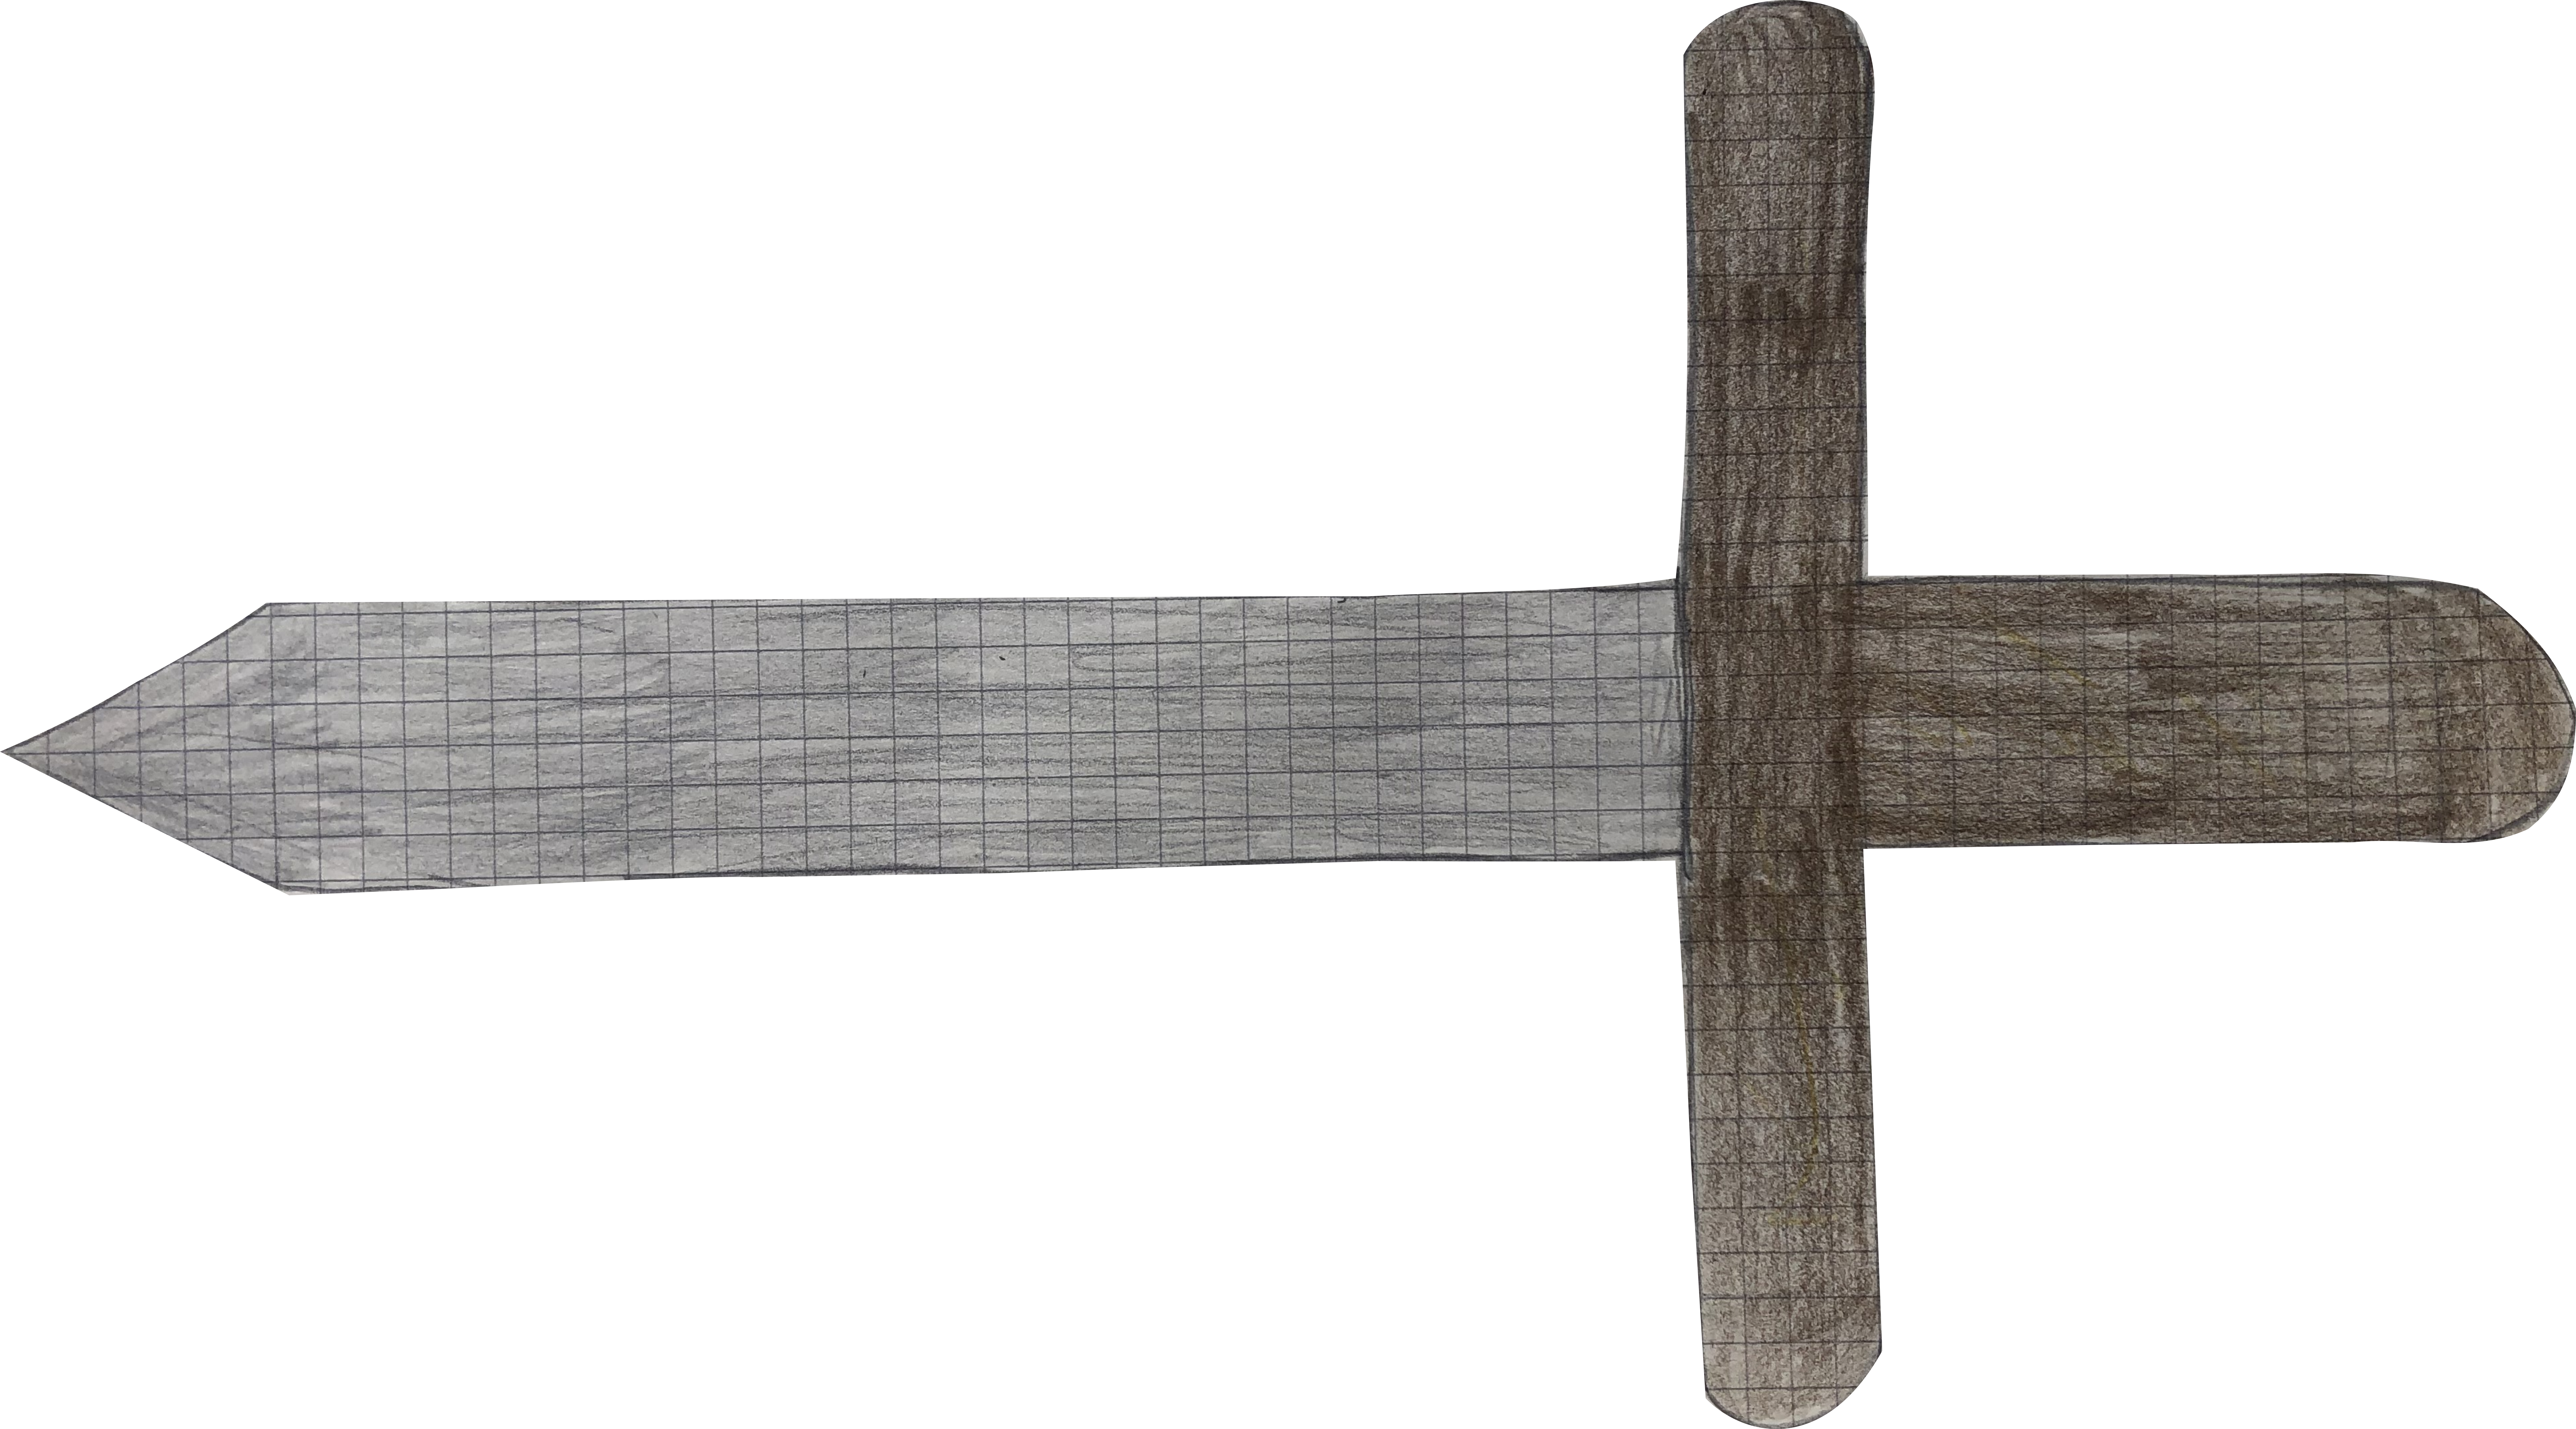
\includegraphics[width=\textwidth]{./bilder/schwert.png}
\end{center}
\vspace*{\fill}
%{\Huge\color{farbe}\hfill{\ttfamily{Fangen}}}
{\centering\fontsize{50}{48} \color{farbe}\sffamily{Sakura}\par}
\addcontentsline{toc}{chapter}{Sakura}
\newpage
%%%%%%%%%%%%%%%%%%%%%%%%%%%%%%%%%%%%%%%%%%%%%%%%%%%%%%%%%%%%%%%%%%%%%%%%%%%%%%%
\lettrine[lines=3, lhang=.2, loversize=.25, lraise=0.05, findent=0.1em,
nindent=0em]{G}{enau} 900 Tage hat die Ausbildung gedauert. Jeden Tag ist Sakura morgens um vier Uhr aufgestanden, um zu trainieren. Die ersten 300 Tage waren der allgemeinen Körperschule und dem Kampf ohne Waffen gewidmet. Eimer mit Wasser füllen und endlose Stufen hoch rennen, hinauf zum Berg Yudonu-san, einem drei heiligen Berge von Dewan, an dessen Fuss die Klosterschule zu Ehren der Göttin Ideah no kami lag. Hier lernte Sakura, ihren Körper in vollkommene Einheit mit ihrem Geist zu bringen, Mediation und Bewegung als Einheit zu begreifen.

Als die erste Stufe abgeschlossen war, erlernte sie die Künste des Kobudō und wurde wegen ihrer Meisterschaft in der Beherrschung des Hanbō, einem schwertähnlichen Stabs ausgewählt, auch die dritte und letzte Stufe der Ausbildung zur Meisterin zu absolvieren, dem Erlernen des Kenjutsu, der Kunst, mit dem Schwert zu kämpfen.

Nicht, dass Sakura gegen jemanden kämpfen wollte, es ging ihr alleine um die vollkommene Beherrschung ihres Körpers und diesen mit einer Waffe zu vereinigen. Also trainierte sie so hart sie konnte. Kraft. Ausdauer. Gelenkigkeit. Und dann die Katas, Bewegungsabläufe bis zur Vollkommenheit beherrschen. Erst hat sie die Bewegungen der Meisterin nur imitiert, aber durch unzählige Wiederholungen dann verstanden. Durch weiter unzählige Wiederholungen schaffte sie es nach den letzten 300 Tagen, eins zu werden, mit diesen Bewegungen. Sie musste nicht mehr an diese Bewegungen denken, das Denken selbst war diese Bewegung.

Und da sie ein ausserordentliches Talent zeigte wurde sie ausgewählt, die Prüfung zur Meisterin abzulegen. Nur einer Schülerin eines Jahrgangs war dies gestattet, die meisten scheiterten. Es war verboten über die Prüfung zu reden, daher wusste niemand als oberste Meisterin, was der Inhalt war. Seit Wochen konnte Sakura nicht mehr schlafen. Was würde es wohl sein? Ein Kampf? Eine Kata?

Und kam der Tag der Prüfung. Gemäss den alten Vorschriften hatte sie seit zwei Tagen nichts gegessen, sondern nur Tee getrunken. Nur sie und die oberste Meisterin befanden sich im hondō, der Grossen Halle des Tempels. Das Sonnenlicht drang nur spärlich durch die Wände aus Reispapier ein.

Nachdem beide zusammen Tee getrunken hatten wie es dem Ritus entsprach, fragte die oberste Meisterin Sokuro, was das Wesen der Schwertkunst in ihren Augen ausmache. Die Einheit zwischen Geist, Körper und Schwert, antwortete sie. Die oberste Meisterin wog ihren Kopf hin und her und liess die Antwort vielleicht gelten. Also gut, antwortete sie. Dann höre, was deine Prüfung ist. Nimm diesen Pinsel und schreibe auf diesem Papier das Zeichen für Einheit. Du darfst darüber meditieren, solange du willst, aber wenn du schreibst, schreibe schnell. Wenn ich in deiner Kalligraphie das Wesen der Schwertkunst erkenne, hast du bestanden.

Damit hätte Sokuro nicht gerechnet. Sie war verunsichert. Schön zu schreiben, war nie ihre Stärke gewesen, immer hatten die Lehrer sie kritisiert. Aber wie es die Oberste Meisterin empfohlen hatte, setzte sie sich hin und meditierte. Sie leerte zunächst ihren Geist, bis die Angst vor der Prüfung, dann die Oberste Meisterin, der Raum und zuletzt sie selbst verschwunden waren. Und als der Geist ganz leer war, meditierte sie über den Schwertkampf. Der Geist führt den Körper, der Körper führt das Schwert. Aber nur das Schwert ist wichtig, also muss das Schwert Teil des Körpers und der Körper Teil des Geistes werden. Nur dann kann ihre Einheit verwirklicht werden. Geschicklichkeit, Kraft und Können. Und genauso verhält es sich auch in der Kalligraphie, nur dass man einen Pinsel, statt eines Schwertes führt.

Und ohne sich von diesem Gedanken zu lösen, stand Sokuro auf, nahm den Pinsel, tauchte seine Spitze in Tinte, wischte ihn vorsichtig ab, schloss die Augen und malte das Zeichen für Einheit, so wie ihr Geist, ihr Körper und der Pinsel es ihr vorgaben. Dann legte sie den Pinsel zurück an seine Stelle, setzte sich zurück auf ihren Platz und löste sich langsam aus ihrer Meditation.

Von dort aus, wo die Oberste Meisterin zugesehen hatte, konnte sie nicht sehen, was Sokuro geschrieben hatte. Sie betrachtete nur die Schülerin. Nach einer Zeit, stand sie auf und verbeugte sich. Das war sehr gut, Meisterin Sokuro sagte sie, du hast die Prüfung bestanden.  \hfill \pgfornament[color=farbe,height=.5cm]{3}

\begin{center}
\includegraphics[width=0.6\textwidth]{./bilder/vereinigung.png}
\end{center}
\newpage
 

